\documentclass[12pt]{article}

%opening
\title{Tesina Segnali e Sistemi 2022}
\author{Lorenzo Franceschetti Mat. 2000263}
\date{}
\usepackage[margin=2cm]{geometry}
\usepackage{graphicx}
\usepackage{float}
\begin{document}

\maketitle

\section{Introduzione}

È dato il segnale $x_{t}(t)$, ottenuto dalla modulazione in ampiezza del segnale $x(t)$ alla frequenza $F_{m}$: 
\begin{equation}
	x_{t}(t) = x(t) cos(2\pi F_{m}t)
\end{equation} 

Studiando il segnale $x_{t}(t)$ in frequenza, ci si aspetta di riconoscere la trasformata $X(f)$ del segnale $x(t)$ centrata in $f = F_{m}$ e la sua speculare centrata in $f = -F_{m}$. Infatti la trasformata $X_{t}(t)$ del segnale modulato in ampiezza con un coseno di frequenza $F_{m}$ risulta essere:
\begin{equation}
	X_{t}(f) = \frac{1}{2}[X(f - F_{m}) + X(f + F_{m})]
\end{equation}

Per ottenere il segnale originale, si ricorre alla seguente procedura:
\begin{itemize}
	\item Si moltiplica il segnale modulato per $2cos(2\pi F_{m}t)$
	\item Si filtra il segnale ottenuto tramite un filtro con risposta in frequenza data da
	\begin{equation}
		H_{lp}(f) = rect \biggl(\frac{f}{2B}\biggr)
	\end{equation}
	con $B$ larghezza di banda monolatera del segnale $x(t)$
\end{itemize}

\section{Studio del segnale modulato}

Il segnale $x_{t}(t)$ e la sua trasformata di Fourier $X_{t}(f)$ risultano essere:
\begin{figure}[H]
	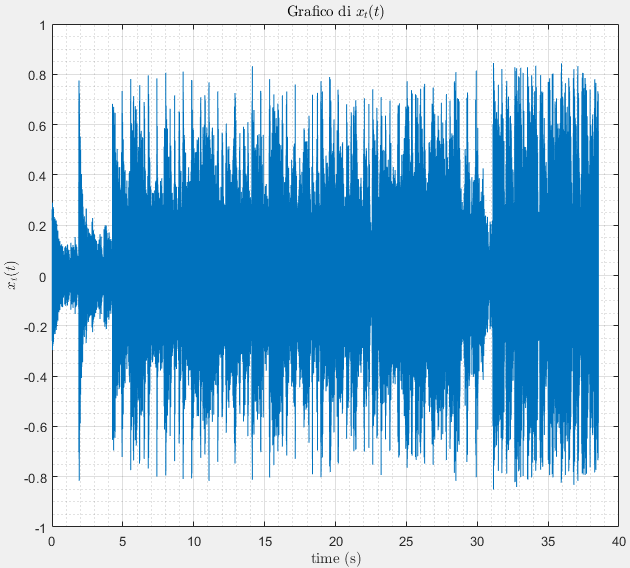
\includegraphics[width=0.5\linewidth]{./images/x_t.png}
	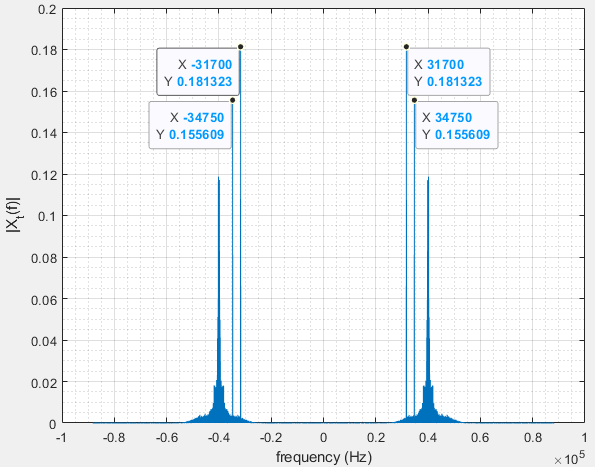
\includegraphics[width=0.5\linewidth]{./images/fft_x_t.png}
\end{figure}

Trascurando per il momento i due picchi a $\pm31700Hz$ e $\pm34750Hz$, il grafico di $|X_{t}(f)|$ mostra due gruppi di componenti, uno per frequenze positive e uno per quelle negative, entrambi simmetrici rispetto all'asse per $f = \pm40000Hz$ rispettivamente, caratteristici della modulazione in ampiezza con un coseno di frequenza $F_{m} = 40000Hz$.

\section{Eliminazione degli artefatti dal segnale}

Il segnale demodulato presenta un disturbo causato da due componenti ad alta frequenza, corrispondenti ai picchi in $\pm31700Hz$ e $\pm34750Hz$ che una volta demodulati si traducono in picchi in $\pm5250Hz$ e $\pm8300Hz$.

Per ridurre il disturbo delle componenti ad alta frequenza, si può adottare un notch filter  in grado di attenuare il segnale in un intervallo molto ristretto di frequenze. Tale filtro è caratterizzato da una frequenza centrale $F_{filter}$, attorno alla quale si sviluppa l'intervallo di attenuazione. Dovendo filtrare due componenti distanti tra loro più dell'ampiezza della banda attenuata del filtro, è necessario impiegare due distinti notch filter, centrati in $F_{filter} = 31700Hz$ e in $F_{filter} = 34750Hz$. 

\section{Campionamento del segnale}

Si procede a campionare il segnale $x(t)$ alla frequenza $F_{c} = 29400Hz$ ricavando il segnale $x_{c}(t)$. All'ascolto si nota la presenza di un disturbo ad alta frequenza, già presente in $x(t)$ e legato alle componenti a $5250Hz$ e $8300Hz$, assieme ad una leggera distorsione del suono legata al fenomeno di aliasing introdotto dal campionamento non ideale. Infatti il segnale $x(t)$ ha una larghezza di banda monolatera pari a $B = 20000Hz$ e viene campionato alla frequenza $F_{c} = 29400Hz$ che non rispetta il requisito $F_{c} > 2B$, violando così una delle ipotesi del teorema di Shannon sul campionamento. Questo comporta che la parte del segnale eccedente la frequenza $\frac{F_{c}}{2} = 14700Hz$ vada a sovrapporsi al segnale utile causando un errore in banda e provocando la leggera distorsione.

\section{Schema alternativo per il campionamento}

Per ridurre l'effetto dei disturbi e quello introdotto dal campionamento si può procedere come segue: 
\begin{itemize}
	\item Si filtra il segnale dato $x_{t}(t)$ con i due notch filter, per sopprimere i disturbi ad alta frequenza, e lo si demodula 
	\item Si applica un filtro passa-basso con frequenza di taglio $F_{st} = 14650Hz$, per ridurre la larghezza di banda del segnale a $B_{\hat{x}_{c}} = F_{st} < \frac{F_{c}}{2}$.  
	\item Si campiona il segnale così ottenuto a $F_{c}$ per avere $\hat{x}_{c}$
\end{itemize}

L'aggiunta del filtro passa-basso consente di rispettare l'ipotesi del teorema di Shannon $F_{c} > 2 B_{\hat{x}_{c}}$ per l'operazione di campionamento ed eliminare l'errore in banda a discapito però di un errore fuori banda, legato alla perdita di informazione delle componenti a più alta frequenza.

\section{Considerazioni sui due metodi}

\begin{figure}[H]
	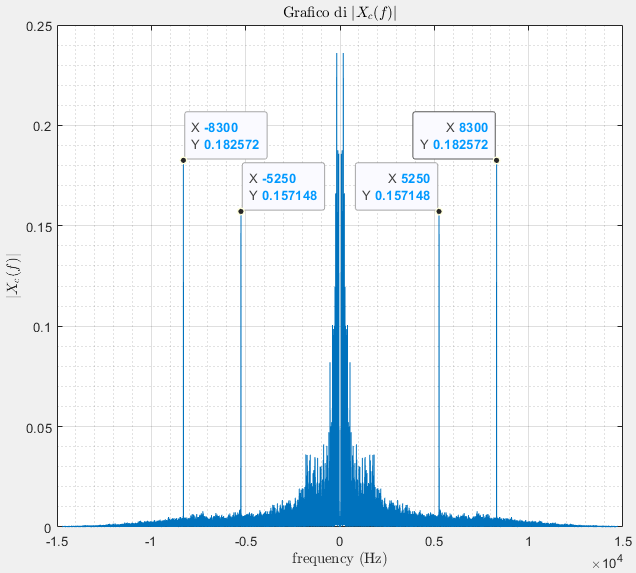
\includegraphics[width=0.5\linewidth]{./images/fft_x_c.png}
	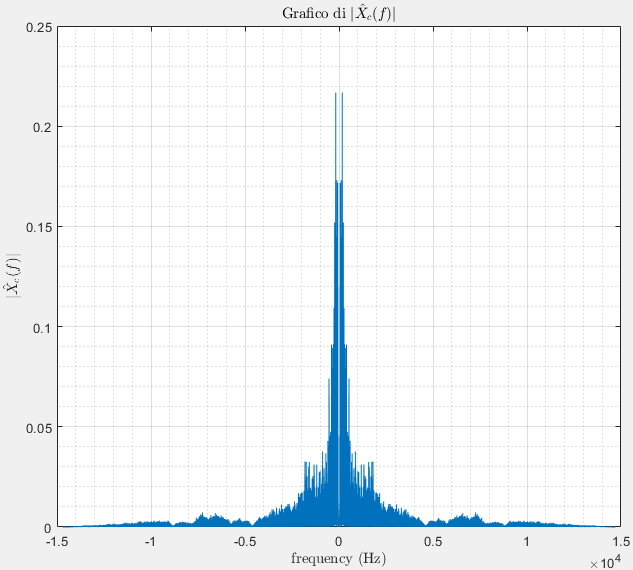
\includegraphics[width=0.5\linewidth]{./images/fft_x_c_hat.png}
\end{figure}

Il segnale $\hat{x}_{c}$ non presenta i disturbi che caratterizzano $x_{c}$, ma perde frequenze alte rispetto al segnale originale. Infatti si nota la scomparsa dei due picchi a $\pm5250Hz$ e $\pm8300Hz$ e, allargando i grafici verso la fine di entrambi gli spettri, si nota come $|X_{c}(f)|$ si interrompe bruscamente a $f = 14700Hz$ e assume in generale valori maggiori di quelli assunti da $|\hat{X}_{c}(f)|$ nella stessa regione. Al contrario, quest'ultima ha una discesa meno brusca, dovuta all'applicazione del filtro passa-basso che attenua fortemente le frequenze al di sopra di $F_{st}$. Scompare dunque il fenomeno di aliasing, e quindi l'errore in banda, nel segnale $\hat{x}_{c}(t)$, al prezzo però di introdurre un errore fuori banda, in quanto si va ad eliminare un intervallo di frequenze.

\end{document}
